\documentclass[a4paper,11pt]{jsarticle}

% 数式
\usepackage{amsmath,amsfonts}
\usepackage{bm}
\usepackage{amsmath,amssymb}
\usepackage{physics}
% 画像
\usepackage[dvipdfmx]{graphicx}
% ボックスなどの装飾
\usepackage{ascmac}

\usepackage{url}
\usepackage[dvipdfmx]{hyperref}

\begin{document}

\title{anyonの別ファイル}
\author{T.S.}
\date{\today}
\maketitle

\section{統計エニオンの第二量子化}
適切な交換関係を決めることによって、統計エニオンは第二量子化をすることができる。

\subsection{トポロジカルエニオンの第二量子化}
まずトポロジカルエニオンについて考えよう。トポロジカルエニオンの生成消滅演算子については、ボソニックまたはフェルミオニックな演算子のJordan-Wigner変換(なんだこれ?)から作られる:
\\

\begin{itembox}[l]{\textbf{Def.トポロジカルエニオンの生成消滅演算子 }}
$\mathcal{C}$を交換のために回す方向で考える閉曲線とする。$a(\vb*{x}_\mathcal{C}),a^{\dag}(\vb*{x}_\mathcal{C})$を$\mathcal{C}$に沿った$\vb*{x}$の消滅,生成演算子とする。
このとき、トポロジカルエニオンの交換関係は次で与えられる。
\begin{align}
a(\vb*{x}_\mathcal{C})a(\vb*{y}_\mathcal{C})-\mathrm{e}^{-i\pi\nu}a(\vb*{y}_\mathcal{C})a(\vb*{x}_\mathcal{C})=0\\
a(\vb*{x}_\mathcal{C})a^{\dag}(\vb*{y}_\mathcal{C})-\mathrm{e}^{i\pi\nu}a^{\dag}(\vb*{y}_\mathcal{C})a(\vb*{x}_\mathcal{C})=0\\
a^{\dag}(\vb*{x}_\mathcal{C})a(\vb*{y}_\mathcal{C})-\mathrm{e}^{i\pi\nu}a(\vb*{y}_\mathcal{C})a^{\dag}(\vb*{x}_\mathcal{C})=0\\
a^{\dag}(\vb*{x}_\mathcal{C})a^{\dag}(\vb*{y}_\mathcal{C})-\mathrm{e}^{-i\pi\nu}a^{\dag}(\vb*{y}_\mathcal{C})a^{\dag}(\vb*{x}_\mathcal{C})=0
\end{align}
\end{itembox}

すなわち、生成同士、消滅同士の交換にはマイナスの位相がかかり、生成と消滅の交換にはプラスの位相がかかる。
トポロジカルエニオンの演算子はブレイド群の表現であるから、交換は時計回りか反時計回りかに依存する。(図1を参照。)
\begin{figure}[htbp]
\begin{center}
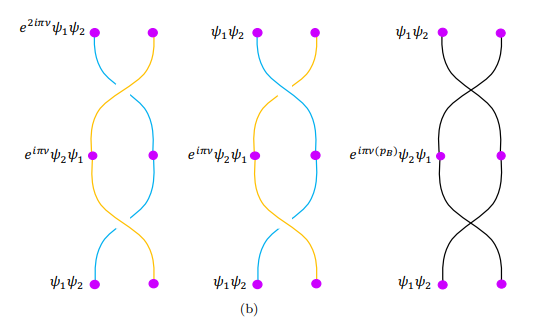
\includegraphics[width=100mm]{braidwf.png}
\caption{ブレイド}
\end{center}
\end{figure}

交換関係を見ると、$\nu=0$でボソンの交換関係を、$\nu=1$でフェルミオンの交換関係を復元することがわかる。
とくに、同じ位置にある粒子においては、エニオニックな位相はキャンセルされ、正準交換関係に帰着する:
\begin{align}
  a(\vb*{x}_\mathcal{C})a^{\dag}(\vb*{x}_\mathcal{C})\pm a^{\dag}(\vb*{x}_\mathcal{C})a(\vb*{x}_\mathcal{C})=1\\
\end{align}
ここで、エニオニックな演算子がフェルミオニックな演算子からきている場合は+、ボソニックな演算子からきている場合は$-$をとる。\\
一般に、トポロジカルエニオンは、$\nu\neq0$のとき、”ハードコアボソン”としてふるまう。ハードコアボソンとは、同じ位置にいない(排他律のある)ボソンである。
この意味で、$\nu$は2つの同一粒子の間の斥力の自由度を定量化していると考えられる。\\
ここの議論は\url{https://www.sciencedirect.com/science/article/pii/055032139390316H}{ A.Lerda, S.Sciuto. Anyons and Quantum Groups}による。

ハードコアボソンの生成消滅演算子$c_i^{\dag}(x_C),c_i(x_C)$を用いて、その議論を追ってみたい。
\begin{align}
  a(\vb*{x}_\mathcal{C})a^{\dag}(\vb*{x}_\mathcal{C})&=K_i(\vb*{x}_C)c_i(\vb*{x})c_i^{\dag}(\vb*{x})K_i^{\dag}(\vb*{x}_C)\\
  &=K_i(\vb*{x}_C)(-c_i^{\dag}(\vb*{x})c_i(\vb*{x})+1)K_i^{\dag}(\vb*{x}_C)\\
  &=-\mathrm{e}^{i\nu\Theta_C(\vb*{x},\vb*{x})}c_i^{\dag}(\vb*{x})K_i(\vb*{x}_c)\mathrm{e}^{i\nu\Theta_C(\vb*{x},\vb*{x})}K_i^{\dag}c_i(\vb*{x})+1\\
  &=-a_i^{\dag}(\vb*{x}_C)a_i(\vb*{x}_C)+1
\end{align}
ただし、
\begin{align}
 K_i(\vb*{x}_C)&=\mathrm{exp}(i\nu\sum_{y\in\Omega}\Theta_{c_{\vb*{x}}}(x,y)c_i^{\dag}(y)c_i(y))\\
K_i^{\dag}(\vb*{x}_C)&=c.c.=K_i^{-1}(\vb*{x}_c)
\end{align}
は、disorder演算子と呼ばれるものである。$\Omega,\Theta$はあとで定義を書くことにする。
これにより中途半端に示された。

\subsection{統計エニオンの第二量子化}
では次に、統計エニオンについて考えよう。
統計エニオンの生成消滅演算子を考えるには、統計エニオンの波動関数を構成したときを思い出せばよい。
量子多体系のHilbert空間として、Fock空間を考える。
そうすると、
\begin{align}
\ket{1}_1\ket{1}_2\dots\ket{1}_N=\prod _{j=1}^{N_B}b_j^{\dag}\ket{0}_j\prod _{k=N_B+1}^{N}f_k^{\dag}\ket{0}_k
\end{align}
と書くことができる。これと同等の表現として統計エニオンの生成演算子を考える:
\begin{align}
  \ket{1}_1\ket{1}_2\dots\ket{1}_N=\prod _{j=1}^{N}s_j^{\dag}\ket{0}_j
\end{align}
演算子$s_j^{\dag}$は、$j\leq N_B$ではボソンの生成演算子に、$N_B\leq j$ではフェルミオンの生成演算子にならなくてはならない。
同様に、消滅演算子も同じ条件を満たさなくてはならない。
この制限のもと、統計エニオンの交換関係は以下のようになる:\\

\begin{itembox}[l]{\textbf{Def.統計エニオンの交換関係 }}
  統計エニオンの交換関係は
\begin{align}
s_j^{\dag}s_j-\mathrm{e}^{i\pi\Theta(j-N_B-1)}s_j s_j^{\dag}=1\\
s_js_j^{\dag}-\mathrm{e}^{i\pi\Theta(j-N_B-1)}s_j^{\dag} s_j=1\\
s_j^{\dag}s_j^{\dag}-\mathrm{e}^{i\pi\Theta(j-N_B-1)}s_j^{\dag} s_j^{\dag}=0\\
s_js_j-\mathrm{e}^{i\pi\Theta(j-N_B-1)}s_j s_j=0
\end{align}
と定義する。
\end{itembox}

1粒子極限を考えると、生成演算子と消滅演算子の関係は

\begin{align}
s_js_j^{\dag}\pm s_j^{\dag}s_j=1
\end{align}

に帰着する。これは、現実にはボソンかフェルミオンかのどちらかであるということを反映している。
また、これは、(5)式の交換関係がフェルミオニックな演算子を元に作られたか、ボソニックな演算子を元に作られたかに依存することを反映している。

\section{統計エニオンと一般化排他統計(Generalized Exclusion Statistics)}
統計エニオンのフェルミオン極限を除いて、統計エニオンとトポロジカルエニオンの注目すべき違いは、排他律がないことである。
かわりに、統計エニオンは”部分的に占有された”状態を許す。
”部分的に占有された状態”というのは、全系の占有率が平均以上の状態である(?)。
この意味で、統計エニオンのフレームワークというのはHaldaneの一般化排他統計(Generalized Exclusion Statistics,GES)に似ている。\\
GESはパウリの排他律を拡張することによって作られたものである。
粒子数を変化させるもとで、量子系のHilbert空間の次元の変化を定量化するパラメタライズされた差分関係(differential relation)を定義することにより拡張された。(この文はまだよくわかっていないのでこんな感じ)
差分関係は

\begin{align}
\Delta  d_{GES}=-g \Delta  N
\end{align}

である。ここで左辺は次元の変化であり、$g$はパラメータだと考えられる。\\
ボソンに対しては、同じ状態を占められる粒子数は無限であるから、次元は粒子数に依存しない。よって$g=0$である。\\
フェルミオンに対しては、排他律のために、それぞれ、追加される粒子によって直接的に次元がスケールされる(粒子がいない次元は考えなくてよいということ?)。よって$g=1$である。\\
GES統計エニオンは、相互作用する気体、たとえばCalogero-Sutherlandモデルなどで見られることが示されている。
驚くべきことに、このGESエニオンの実現は、最低Landau準位に閉じ込められたトポロジカルエニオンに直接マッピングできる。
GESエニオンは、極低温Hubberdチェインと同様に、Calogero-SutherlandモデルやLieb-Linigerモデル、ハードコアTonks-Girardeau気体などに見られている。
もっと一般に、GESに従う理想準粒子の観点から、熱力学的Bethe仮設によって計算しなおせる可積分モデルの存在が示されている。\\
この統計エニオンのフレームワークでは、統計エニオンのHilbert空間の次元変化はボソンの次元変化とフェルミオンの次元変化の和で与えられる。
それぞれの出現確率$p_B,p_F$を用いて、
\begin{align}
\Delta d_{SA}=p_B\Delta d_b+p_F\Delta d_F
\end{align}
とかける。
$\Delta d_B=0,\Delta d_F=-\Delta N$のとき、$\Delta d_{SA}=-p_F\Delta N$と単純になる。
はじめの式と一つ上の式を見比べると、GESのフレームワークにおけるパラメータ$g$というのは、統計エニオンのフレームワークにおけるフェルミオンの出現確率によってきまってしまうということがわかる。
これは統計エニオンのフレームワークがGESエニオンのフレームワークとまったく同等であることを示している。
GESエニオンはボソンとフェルミオンの観点から説明できることは、MurthyとShankerが、Calogero-Sutherlandモデルは理想GESエニオンであることを指摘した際にわかった。
その結果、分配関数はボソニックな部分とフェルミオニックな部分に分けられ、それぞれ、GESパラメータ$g,g-1$の累乗で構成されることがわかった。
これにより、GESはボソンとフェルミオンの理想敵な混合であることが指摘された。\\
統計エニオン、GESエニオンは任意の次元で実現できる(次元に一般的な制限はない)というのは、トポロジカルエニオンとの大きな違いである。


\section{エニオンの平衡熱力学}
\subsection{1次元統計エニオン}
エニオン系の熱力学を理解するためにまず考えることは、熱力学量にエニオンの位相がどのように依存するかである。
これをきめるために、適切な分配関数を導入する。トラップされた相互作用するGESガスの実現でモチベートされたように、1次元調和ポテンシャル中の2つの統計エニオンを考えよう。\\
しかし、この際、我々は相互作用しない粒子系を考えている。
(GESは単なる混合でよいのか?)
トラップされたボソンーフェルミオン混合物は以前より、理論的あるいは実験的に研究されているが、この研究ではおもに、基底状態の設定でボソン、フェルミオン間の相互作用から生じる効果に焦点を当てよう。
統計エニオンのフレームワークでは我々は、混合物の代わりに、そのような混合の理想気体極限として多体平均のふるまいを考える。
調和ポテンシャル中に閉じ込められた2つの統計エニオンのハミルトニアンは

\begin{align}
H=\frac{p_1^2+p_2^2}{2m}+\frac{1}{2}m\omega^2(x_1^2+x_2^2)
\end{align}
で与えられる。統計エニオンののフレームワークでは、ハミルトニアンのもとで発展するエニオンのペアの分配関数というのは
\begin{align}
Z_{SA}=(Z_B)^{p_B}(Z_F)^{1-p_B}
\end{align}
となる。ここで、それぞれの粒子の分配関数を$Z_i,i=B,F$とした。元論文の付録Aにはこの分配関数の導き方が書いてあるので余裕があるときに読む。
この分配関数は、CSmodelの$g\rightarrow1-p_B$としたものに等しい。
我々はここに、統計エニオンの枠組みの中では、エニオニックなふるまいというのは、ハミルトニアンの中の相互作用項からというよりむしろ、平均の性質の上で純粋に現れるのである。(CSmodelをもっと見てみる必要があるよこれは)
この分配関数を使うと、熱力学的な量はただちに導かれる。
分配関数を実際に代入してみると、

\begin{align}
E=\frac{1}{2}\hbar \omega[3\coth (\beta\hbar\omega)+\csch(\beta\hbar\omega)-2p_B+1 ]
\end{align}








\end{document}